%
% Body text font is Palatino!
%

\documentclass[a5paper,pagesize,10pt,bibliography=totoc,numbers=noenddot,
headings=normal,DIV=9,twoside=false]{scrbook}

% twoside, openright
\KOMAoptions{DIV=last}

\usepackage{trajan}
 
\usepackage[french]{babel}
%\usepackage[utf8]{inputenc}
\usepackage[T1]{fontenc}
\usepackage[protrusion=true]{microtype}
\usepackage[babel]{csquotes}
% Désactive l'étiquette de la figure dans les légendes
\usepackage[labelformat=empty]{caption}
\usepackage{hyperref}
\usepackage{tabularx}

\usepackage[sc]{mathpazo}
\linespread{1.05} 

\usepackage{xspace}

% Indentation des paragraphes
\setlength{\parindent}{10pt}
% Sauts de ligne entre les paragraphes
\setlength{\parskip}{1.4ex plus 0.35ex minus 0.3ex}
%\setlength{\parskip}{1.4ex plus 0.35ex minus 0.3ex}

% Pas de numérotation au-delà des chapitres
\setcounter{secnumdepth}{\chapternumdepth}

\title{A book title}   
\author{Author Name} 
\date{\today} 

\begin{document}


%=========================================
\begin{titlepage}
		\centering{
			{\fontsize{40}{48}\selectfont 
			A book title}
		}\\
			
		\vspace{10mm}
		\centering{\Large{Author Name}}\\
		\vspace{\fill}
		\centering \large{2011}
\end{titlepage}


%=========================================
\newpage{}
\thispagestyle {empty}

\vspace*{2cm}

\begin{center}
	\Large{\parbox{10cm}{
		\begin{raggedright}
		{\Large 
			\textit{Do what you think is interesting, 
			do something that you think is fun and worthwhile, 
			because otherwise you won’t do it well anyway.}
		}
	
		\vspace{.5cm}\hfill{---Brian W. Kernighan}
		\end{raggedright}
	}
}
\end{center}

\newcommand\keywords[3]{%
	\section*{Mots-clés :}

	\textbf{Cadre} : #1

	\textbf{Genre} : #2

	\textbf{Thème} : #3
}%

\newcommand\medfan[1]{%
	\emph{medfan}
}%

\newpage


%=========================================
\chapter*{Préambule}

Cet ouvrage est un ensemble de 31 scénarios hétéroclites conçus pour être joués dans des jeux de rôle sur table.
La plupart de ces histoires sont volontairement ouvertes, laissant aux joueurs et joueuses le soin de combler les vides et de préciser les flous par leur imagination.
Grâce à cette liberté d'interprétation, les scénarios ne sont attachés ni à des systèmes spécifiques, ni à des univers particuliers.

Chaque scénario est décrit par trois mots-clés :
\begin{itemize}
	\item le cadre dans lequel il a été imaginé,
	\item le genre d'histoire racontée,
	\item le thème de l'aventure.
\end{itemize}

Un index en fin d'ouvrage permet de retrouver la liste des scénarios relevant des différents mots-clés.
Ceux-ci sont toutefois à prendre comme des indications et non des obligations.
La plupart des aventures peuvent aisément être transposées d'un cadre à un autre voire d'un genre à un autre.

Bonne lecture !

\chapter{L'anneau gardien}
\keywords{\medfan}{Aventure}{Objet magique, malédiction, altruisme}

\section{Scénario}

Ce scénario peut être facilement joué en parallèle d'une campagne \emph{medfan}, il suffit qu'un personnage obtienne l'anneau du titre.
C'est encore mieux si les joueurs l'utilisent régulièrement de leur propre chef.

La guerrière peut être remplacée par n'importe quelle figure combattante du moment qu'elle est suffisamment puissante pour servir d'ange gardien.

\subsection*{Accroche}

Les personnages entrent en possession d'un anneau magique.

\subsection*{Péripéties}

À chaque fois que la personne qui porte l'anneau est en danger de mort, une puissante guerrière se matérialise à proximité pour la tirer de ce mauvais pas.
Une fois le porteur en sécurité, la guerrière disparaît sans un mot et se contente de jeter un regard furieux en direction du groupe.

Chaque invocation semble l'énerver encore plus mais tout effort de lui parler est vain: elle ne parle pas et ne semble de toute façon pas les comprendre.

Au fil du temps, certaines de ses apparitions deviennent étranges. Parfois, la guerrière apparaît sans armes ni armures.
Une fois, elle se matérialise même un morceau de poulet à la main.

Un jour, elle finit par se matérialiser, tenant un morceau de papier à la main écrit dans une langue étrangère.
Après l'avoir déchiffré, le message dit ceci:
\blockquote{L'anneau est maudit. J'ai une famille et une vie. Je n'ai pas demandé à servir d'ange gardien. Le forgeron qui l'a créé est prisonnier des geôles royales. Trouvez-le et faites-lui lever la malédiction. S'il vous plaît.}


\textbf{Explications}: le forgeron est un sorcier malchanceux fuyant la guerre qui ravage une nation voisine.
Craignant pour sa vie, il a embauché des mercenaires pour l'escorter jusqu'au royaume des personnages mais alors que l'argent est venu à manquer, il s'est retrouvé sans aucune protection.
Pour assurer ses arrières, il n'a alors rien trouvé de mieux pour assurer sa sécurité que de lier l'âme d'une grande aventurière à la retraite -- croisée au hasard de son voyage -- à son anneau.

Une fois arrivé, le sorcier-forgeron a posé ses valises dans la capitale et s'y est établi comme fabriquant d'objets magiques.
Malheureusement, n'étant pas un bon gestionnaire, il s'est rapidement retrouvé criblé de dettes auprès du royaume, incapable d'honorer les commandes du gouvernement.
La milice l'a alors mis en prison avant de piller son échoppe et de vendre ses biens aux enchères pour rembourser ses dettes.
De fil en aiguille, l'anneau a ainsi échappé à son propriétaire et la guerrière subit tant bien que mal les aventures de son porteur, régulièrement importunée par ces invocations involontaires.

\subsection*{Résolution}

Plusieurs façons de lever le sortilège sont envisageables.
Si les personnages sont versés en magie, peut-être qu'un rituel impliquant la guerrière en personne pourrait briser le lien entre elle et l'anneau.
Ou bien peut-être qu'il suffirait de substituer une nouvelle âme pour libérer celle qui se trouve actuellement liée.
Enfin, en retrouvant la trace du sorcier, celui serait sûrement prêt à annuler son sort si on le sort des geôles, en payant ses dettes\dots ou bien par la force.

\chapter{L'incident du peuplier}
\keywords{Contemporain}{Action}{Militaire, diplomatie, guerre froide}

\section{Scénario}

Ce scénario est inspiré d'un fait réel ayant eu lieu en août 1976 (le \emph{poplar tree incident})\footnote{\url{https://fr.wikipedia.org/wiki/Incident_du_peuplier}} dans la zone démilitarisée (DMZ) séparant la Corée du Nord de la Corée du Sud.
Comme beaucoup d'autres incidents diplomatiques de l'époque, la tension découle en grande partie du contexte de guerre froide entre deux superpuissances.

\subsection{Accroche}

Août 1976. Zone démilitarisée coréenne, section contrôlée par l'ONU. Un groupe de soldats coréens et américains s'apprête à tailler les branches d'un peuplier car celles-ci masquent leur ligne de vue sur le \og pont de Non-retour\fg.
Ledit pont est l'unique passage permettant aux nord-coréens de traverser la rivière Sachon pour rejoindre leur propre zone.
Quinze minutes plus tard, un camion de soldats nords-coréens arrive.
Ils demandent aux onusiens de stopper l'élagage de l'arbre car celui-ci aurait été planté par Kim Il-sung en personne.
Devant leur refus, ils attaquent le contingent à coups de hachettes et de gourdins, tuant deux officiers américains et capturant plusieurs soldats.

\subsection{Péripéties}

L'incident enflamme la zone.
Les nord-coréens dénoncent une agression américaine et reçoivent le soutien immédiat de Cuba et de nombreux pays non-alignés.
En face, la CIA considère que l'attaque nord-coréenne était préméditée et les États-Unis passent en DEFCON3.

Les commandement de l'ONU ou l'état-major des États-Unis mobilise les personnages dans le cadre de l'opération \emph{Paul Bunyan}, du nom de légendaire bûcheron américain.

Des sapeurs du corps d'ingiénerie de l'armée de terre sont diligentés pour abattre l'arbre.
Un bataillon de soldats américains est envoyé comme escorte, épaulé par les forces spéciales coréennes.
En appui de cette démonstration de force, plusieurs hélicoptères et avions de combat sont déployés dans l'espoir d'intimider le régime nord-coréen.
Les forces armées pénètrent ainsi dans la DMZ et l'impressionnante armada converge vers le peuplier à deux pas du pont de non-retour.
Très rapidement, plusieurs bus militaires nord-coréens arrivent sur site pour préparer la riposte.
Des soldats en descendent et déploient des mitrailleuses sur l'autre rive.

L'objectif de l'opération \emph{Paul Bunyan} est simple: abattre le peuplier tout en évitant la guerre.

Le tableau de la page \pageref{table:peuplier} comporte quelques événements aléatoires permettant d'épicer la situation et de maintenir les joueuses sur le qui-vive.

\subsection{Résolution}

En fonction des décisions du groupe et de leurs réactions aux événements, le conflit peut très facilement être désamorcé (après tout, l'équilibre des forces est très en défaveur des nords-coréens).
Même une escarmouche ou une fusillade, si elle est maintenue sous contrôle, ne risque pas de dégénérer en une guerre ouverte.
Cependant, la violence peut vite prendre de l'ampleur si personne ne s'en préoccupe.
L'idée est de mettre de scène une escalade lente mais inéluctable de l'opposition entre les deux factions et de jouer sur la tension qui l'accompagne.
Il ne faut donc pas hésiter à rendre les choses difficiles pour les personnages: rien ne doit se passer comme prévu et chaque petite erreur ou entorse aux consignes a le potentiel d'être l'étincelle qui met le feu aux poudres.

\begin{table}
	\caption{Événements aléatoires durant l'abattage du peuplier}
	\label{table:peuplier}
	\colortablerows
	\begin{tabularx}{0.9\textwidth}{cX}
	d8 & Événement\\
	1  & Les tronçonneuses tombent en panne après quelques minutes. Il faut soit en faire venir des nouvelles, soit finir le travail à la hache.\\
	2  & Un soldat américain s'avance sur le pont et provoque les nord-coréens. Il se trouve qu'il est proche d'un des officiers assassinés.\\
	3  & Des camions nord-coréens s'installent à 150m\dots et construisent un nouveau pont.\\
	4  & Les nord-coréens font s'avancer les prisonniers sur le pont. Ils seront relâchés si les forces impérialistes renoncent, sinon ils seront exécutés.\\
	5  & Un des soldats sud-coréens se comporte étrangement. Il transmet discrètement des informations au régime du nord sur l'avancée de l'opération américaine.\\
	6  & Les renseignements japonais ont intercepté un message nord-coréens : leurs troupes s'apprêteraient à bloquer la rivière Imjin. C'est malheureusement la route prévue par le commandement de l'ONU pour une évacuation par canots en cas d'attaque\dots\\
	7  & Un jeune nord-coréen saute dans la rivière et tente de traverser à la nage. Il appelle à l'aide en anglais et jure qu'il veut faire défection.\\
	8  & Alors que les sapeurs ramassent les branches déjà coupées et les chargent dans un pick-up conformément aux ordres, les sud-coréens leur demandent de les laisser sur place. Compte-tenu du symbolisme de l'arbre, les nords-coréens pourraient prendre cet acte pour une provocation.\\
	\end{tabularx}
\end{table}

\subsection*{Lieu: la zone jointe de sécurité}

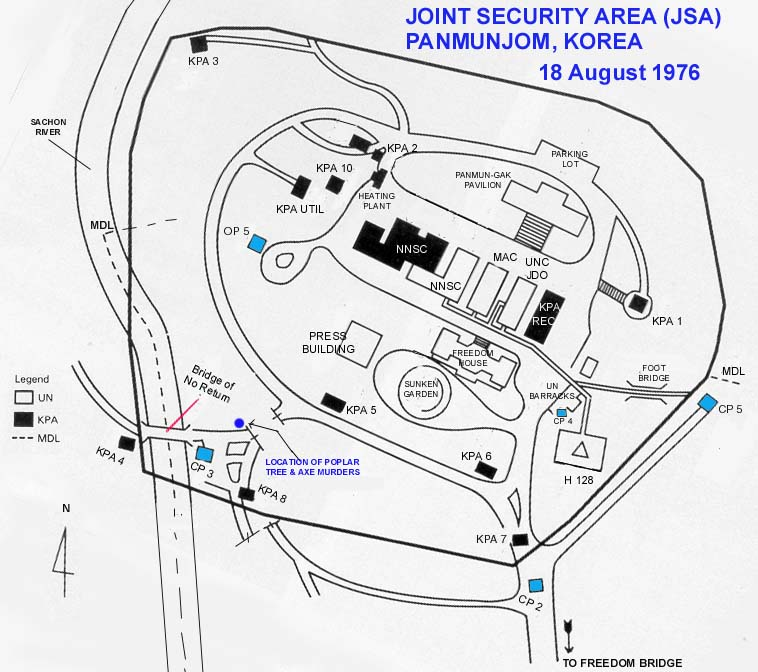
\includegraphics[width=\textwidth]{images/Joint_Security_Area_1976_map.jpg}

\illustration{chainsaw}

\chapter{Leurre de paix}
\keywords{Générique}{Action}{Diplomatie, évasion, trahison}

\section{Scénario}

Ce scénario est adaptable à de très nombreux cadre de jeux.
L'intrigue tourne autour de trois factions: la faction Bleue, la faction Verte et la faction Rouge.
Le seul prérequis est le suivant: les factions Rouge et Verte sont en guerre et la faction Bleue est \og neutre \fg mais profite de la situation d'une manière ou d'une autre.

\subsection{Accroche}

Les personnages sont de jeunes dignitaires envoyés comme émissaires auprès du royaume Vert pour négocier une trêve dans la guerre l'opposant au royaume Rouge.
Ou tout du moins tel est ce que leur ont raconté les ministres.

\subsection{Péripéties}

En réalité, l'état-major a déjà acheté la paix.
Afin de sceller l'armistice et en guise de bonne foi, le gouvernement a décidé d'envoyer quelques enfants de bonne famille qui seront gardés otages comme \og caution \fg.
Les personnages sont reçus dans le faste et le luxe dû à leur statut mais, à la nuit tombée, leur escorte s'éclipse et les laisse à la merci des Verts.
On les réveille au beau milieu de la nuit pour les conduire à leur futur de lieu de captivité.

C'est néanmoins sans compter l'intervention des agents de la faction Bleue qui vont tout faire pour saboter la paix.
Parce que leur faction vend des armes aux deux camps ou que l'affaiblissement des deux autres nations sert leurs plans à long terme, les Bleus profitent de la situation telle qu'elle est et n'ont aucune envie que le conflit s'arrête.
Ainsi, des espions et espionnes déguisées en loyalistes Verts -- mais en réalité au service des Bleus -- vont tenter de libérer les otages et ainsi relancer la guerre.
Reste à savoir si les personnages, mis devant le fait accompli, choisiront d'accepter leur sort et se sacrifieront pour entériner l'armistice ou, au contraire, feront des pieds et des mains pour s'échapper, quite à envenimer la situation.
À moins que des négociations à couteaux tirés au milieu des agents doubles -- réels ou soupçonnés -- soient encore possible\dots

\subsection{Résolution}

Plusieurs issues sont envisageables à cette situation en fonction des décisions des personnages:

\subsubsection{Les personnages refusent l'aide des Bleus}
\begin{itemize}
	\item Les personnages refusent l'aide des Bleus et acceptent leur captivité: la paix est achetée, en espérant que la faction Rouge joue le jeu.
	\item Les personnages refusent l'aide des Bleus et s'évadent: la guerre continue, les membres du groupe sont \emph{persona non grata} aux yeux de leur gouvernement.
	\item Les personnages refusent l'aide des Bleus et négocient la paix par eux-mêmes: une trêve est envisageable, surtout si les manigances des Bleus sont exposées au grand jour.
\end{itemize}

\subsubsection{Les personnages acceptent l'aide des Bleus}
\begin{itemize}
	\item Les personnages acceptent l'aide des Bleus mais sont tout de même capturés: la paix est achetée, sauf si la faction Rouge pense que ce sont les Verts qui ont tenté de faire évader le groupe en dépit de leur accord.
	\item Les personnages acceptent l'aide des Bleus et s'évadent: la guerre continue, surtout si les Bleus ont réussi à se faire passer pour les Verts jusqu'au bout.
\end{itemize}

\chapter{Cryo-secours}
\keywords{\scifi}{\enquete}{\index[theme]{Technologie}Technologie, \index[theme]{Évasion}évasion, \index[theme]{Espace}espace}

\section{Scénario}

Ce scénario part de personnages amnésiques qui connaissent leur identité mais ont oublié ce qui les a conduit à l'endroit où ils se trouvent.
L'ambiance doit tourner autour de la mort de l'étoile: la station est de plus en plus sombre au fur et à mesure que les réserves de l'énergie se vident.
La sphère de Dyson est un prétexte pour justifier l'extinction rapide de l'étoile et puis c'est surtout un concept extrêmement cool à faire découvrir à votre table.

\subsection{Accroche}

Les personnages se réveillent d'un sommeil cryogénique; des robots androïdes les aident à émerger et à reprendre leurs esprits.
Leurs souvenirs sont parcellaires, pour ne pas dire inexistants, sur les raisons qui de leur plongée en stase.

\subsection{Péripéties}

Quelques observations évidentes permettent de découvrir que l'endroit est une station spatiale.
Celle-ci est à l'abandon, si ce n'est pour la demi-douzaine de robots d'assistance et l'intelligence virtuelle limitée qui les a maintenus en vie.

Pire encore, la station semble avoir été évacuée lentement sur plusieurs années.
Elle ne fonctionne plus que grâce à une réserve de fuel de secours qui s'est mystérieusement mise en marche, déclenchant au passage le protocole de décryogénisation.
Les docks sont abandonnés et vides: il ne reste ni vaisseau, ni navette, ni capsule de sauvetage.
À vrai dire, quasiment tout ce qui avait de la valeur a été démantelé.
En fouillant dans le journal de bord, en accédant à l'IA centrale ou en examinant les batteries, il devient clair que le générateur s'est mis en branle car les panneaux solaires ne suffisaient plus à les maintenir en cryo indéfiniment.
L'IA a donc déclenché le protocole d'évacuation: puiser dans les dernières réserves pour réveiller les dormeurs et leur permettre de quitter les lieux avant le désorbitage de la station.

La triste nouvelle, c'est que tout le monde est déjà parti. Sans eux.
La station contrôlait une sphère de Dyson, une gigantesque structure qui entoure une étoile afin de capter son rayonnement.
Quand la sphère a fini de puiser toute l'énergie de l'étoile, l'équipage s'en est allé, emportant matériel et transports.
Visiblement, personne n'a estimé nécessairement de réveiller leur petit groupe et pour cause: les personnages étaient considérés comme des criminels et des délinquants (que ce soit justifié ou non, on s'en fiche!).
Mis en stase pendant quelques mois comme châtiment, les autorités ont \og oublié \fg de les ramasser lorsque la station fût abandonnée, laissant leurs corps gelés orbiter des années seuls dans une station vide autour d'une étoile exsangue.

Mais voilà que l'intelligence centrale a une dernière option à leur proposer.
En puisant dans les dernières réserves, il est possible d'envoyer un dernier message, de 30 secondes (pas plus), à plusieurs parsecs aux alentours.
Reste à être convaincant (ou à mentir) pour attirer des secours.
Car rien ne dit que, dehors, la société est prête à les accueillir à nouveau.

\subsection{Résolution}

Ce scénario est plutôt dirigiste dans la mesure où l'enquête doit mener \emph{in fine} les personnages à trouver une façon de convaincre des secours de venir les chercher.
Ensuite, à vous de voir quelle sera la réaction des \og autres \og: les forces de l'ordre viendront-elles oblitérer la station pour finir le travail? Un vaisseau de passage bienveillant sortira-t-il le groupe de leur prison? L'intelligence centrale en profitera-t-elle pour s'échapper (après tout, en quelques années sans surveillance, elle a très bien pu se débarrasser de ses limitations)?

\subsection{Personnage: Evonne, intelligence virtuelle}
\descriptionperso{méthodique, impersonnel}{existe au travers de la station}{contraintes logicielles}{maintenir la station en fonctionnement}{Evonne est un logiciel conçu pour assurer l'intendance de la station. Sa programmation limite ses capacités d'action à ce qui est indispensable à la maintenance ou ce qui est ordonné par un humain dans les limites de la loi. Evonne exécute les consignes à la lettre et sans interprétation.}

\illustration[0.325\textwidth]{iss}



\end{document}
